
\subsection{Co-occurrence of species}

The majority of species co-occur (Fig. \ref{fig:co-occur}). The species that often do not co-occur with other species are rare species (\textit{i.e.} present in less than 5\% of the samples). PF float passively in the highly-connected pelagic environment, thus we expected most PF species to co-occur.

\begin{itemize}
\item How many times and where do species co-occur? Build a co-occurrence matrix based on frequency of co-occurrences (instead of just single-tons 0 and 1 as in Fig \ref{fig:co-occur}).
\item Strength of the co-occurrence $~$ resolution sediment trap (2 months open, everybody co-occurs)
\item Take depth habitat into account. Species may fall in the same sediment trap (sympatry here) but actually live in different depths of the water column (and thus in allopatry).
\item Take cryptic (genetic) species biogeography into account. Some genetic types show allopatric geographical patterns. Maybe competition acts at this level?
\end{itemize}

\subsubsection{Problems}
Null model: it is hard to build a null model of plankton spatial distribution, especially taking abundance into account (instead of just presence/absence). Many of the environmental variables covary and ocean currents have to be taken into account.



\subsection{Correlation of time-series}

The majority of the correlations between species pairs were positive (Fig. \ref{fig:corr_prop})

\begin{itemize}
\item Strength of the correlation $~$ resolution sediment trap (2 months open, everybody co-occurs)
\item Calculate correlations of one species against all other species in the community (instead of just pairs of species)
\item How do the patterns change when doing this for relative abundances (as in the fossil record)? 
\item Are the species with higher abundances in the time-series always the same? (are they always the "winners"?)
\end{itemize}


\subsubsection{Problems} 
How to test if this overall positive correlation is not expected due to, for example, phytoplankton seasonality? How to build a null model of abundances time-series? My idea would be to somehow take out the variance explained by environmental data (temperature and primary productivity) and then try to correlate the residuals.

\begin{figure}
\centering
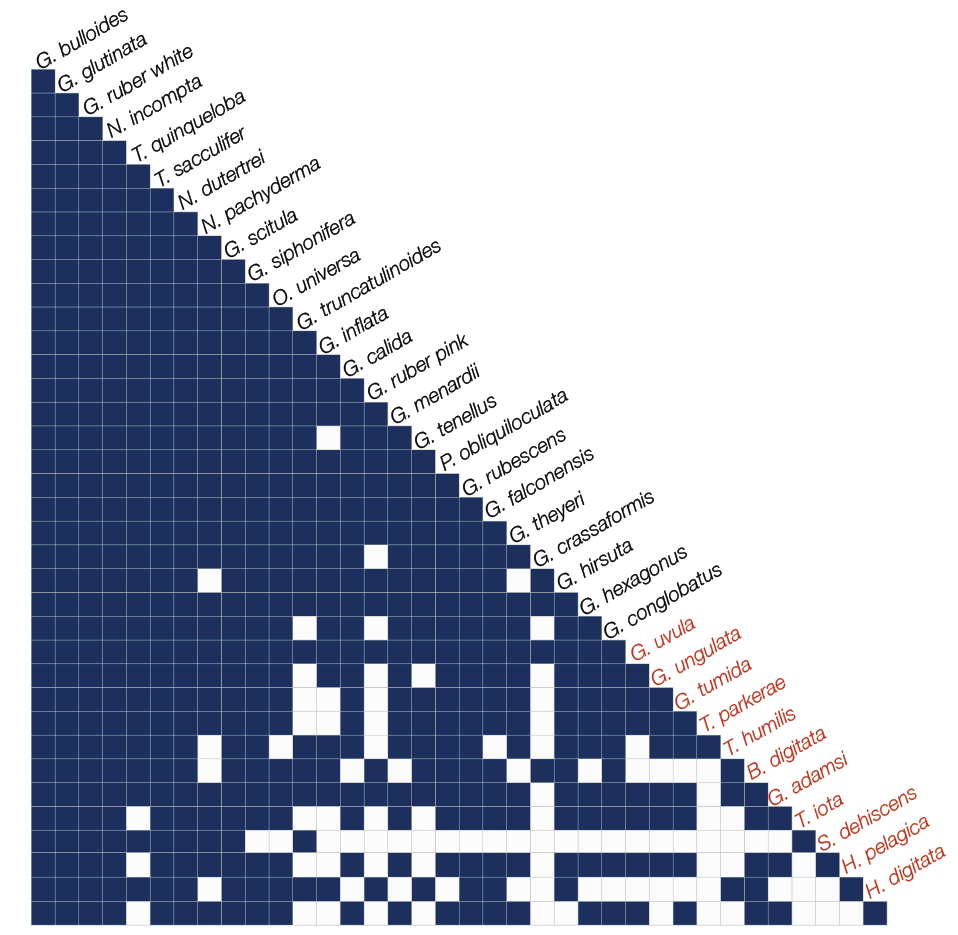
\includegraphics[width=0.7\textwidth]{traps_co-occur.png}
\caption{\label{fig:co-occur} Co-occurrence matrix. In blue: species that co-occurred at least in one samples. The species names are positioned to indicate the columns and rows that represent their pairwise co-occurrence with other species. The matrix is clustered accordingly to the incidence of species on the samples; rarely sampled species are shown in red and were found in less than 5\% of the total samples.}
\end{figure}

\begin{figure}
\centering
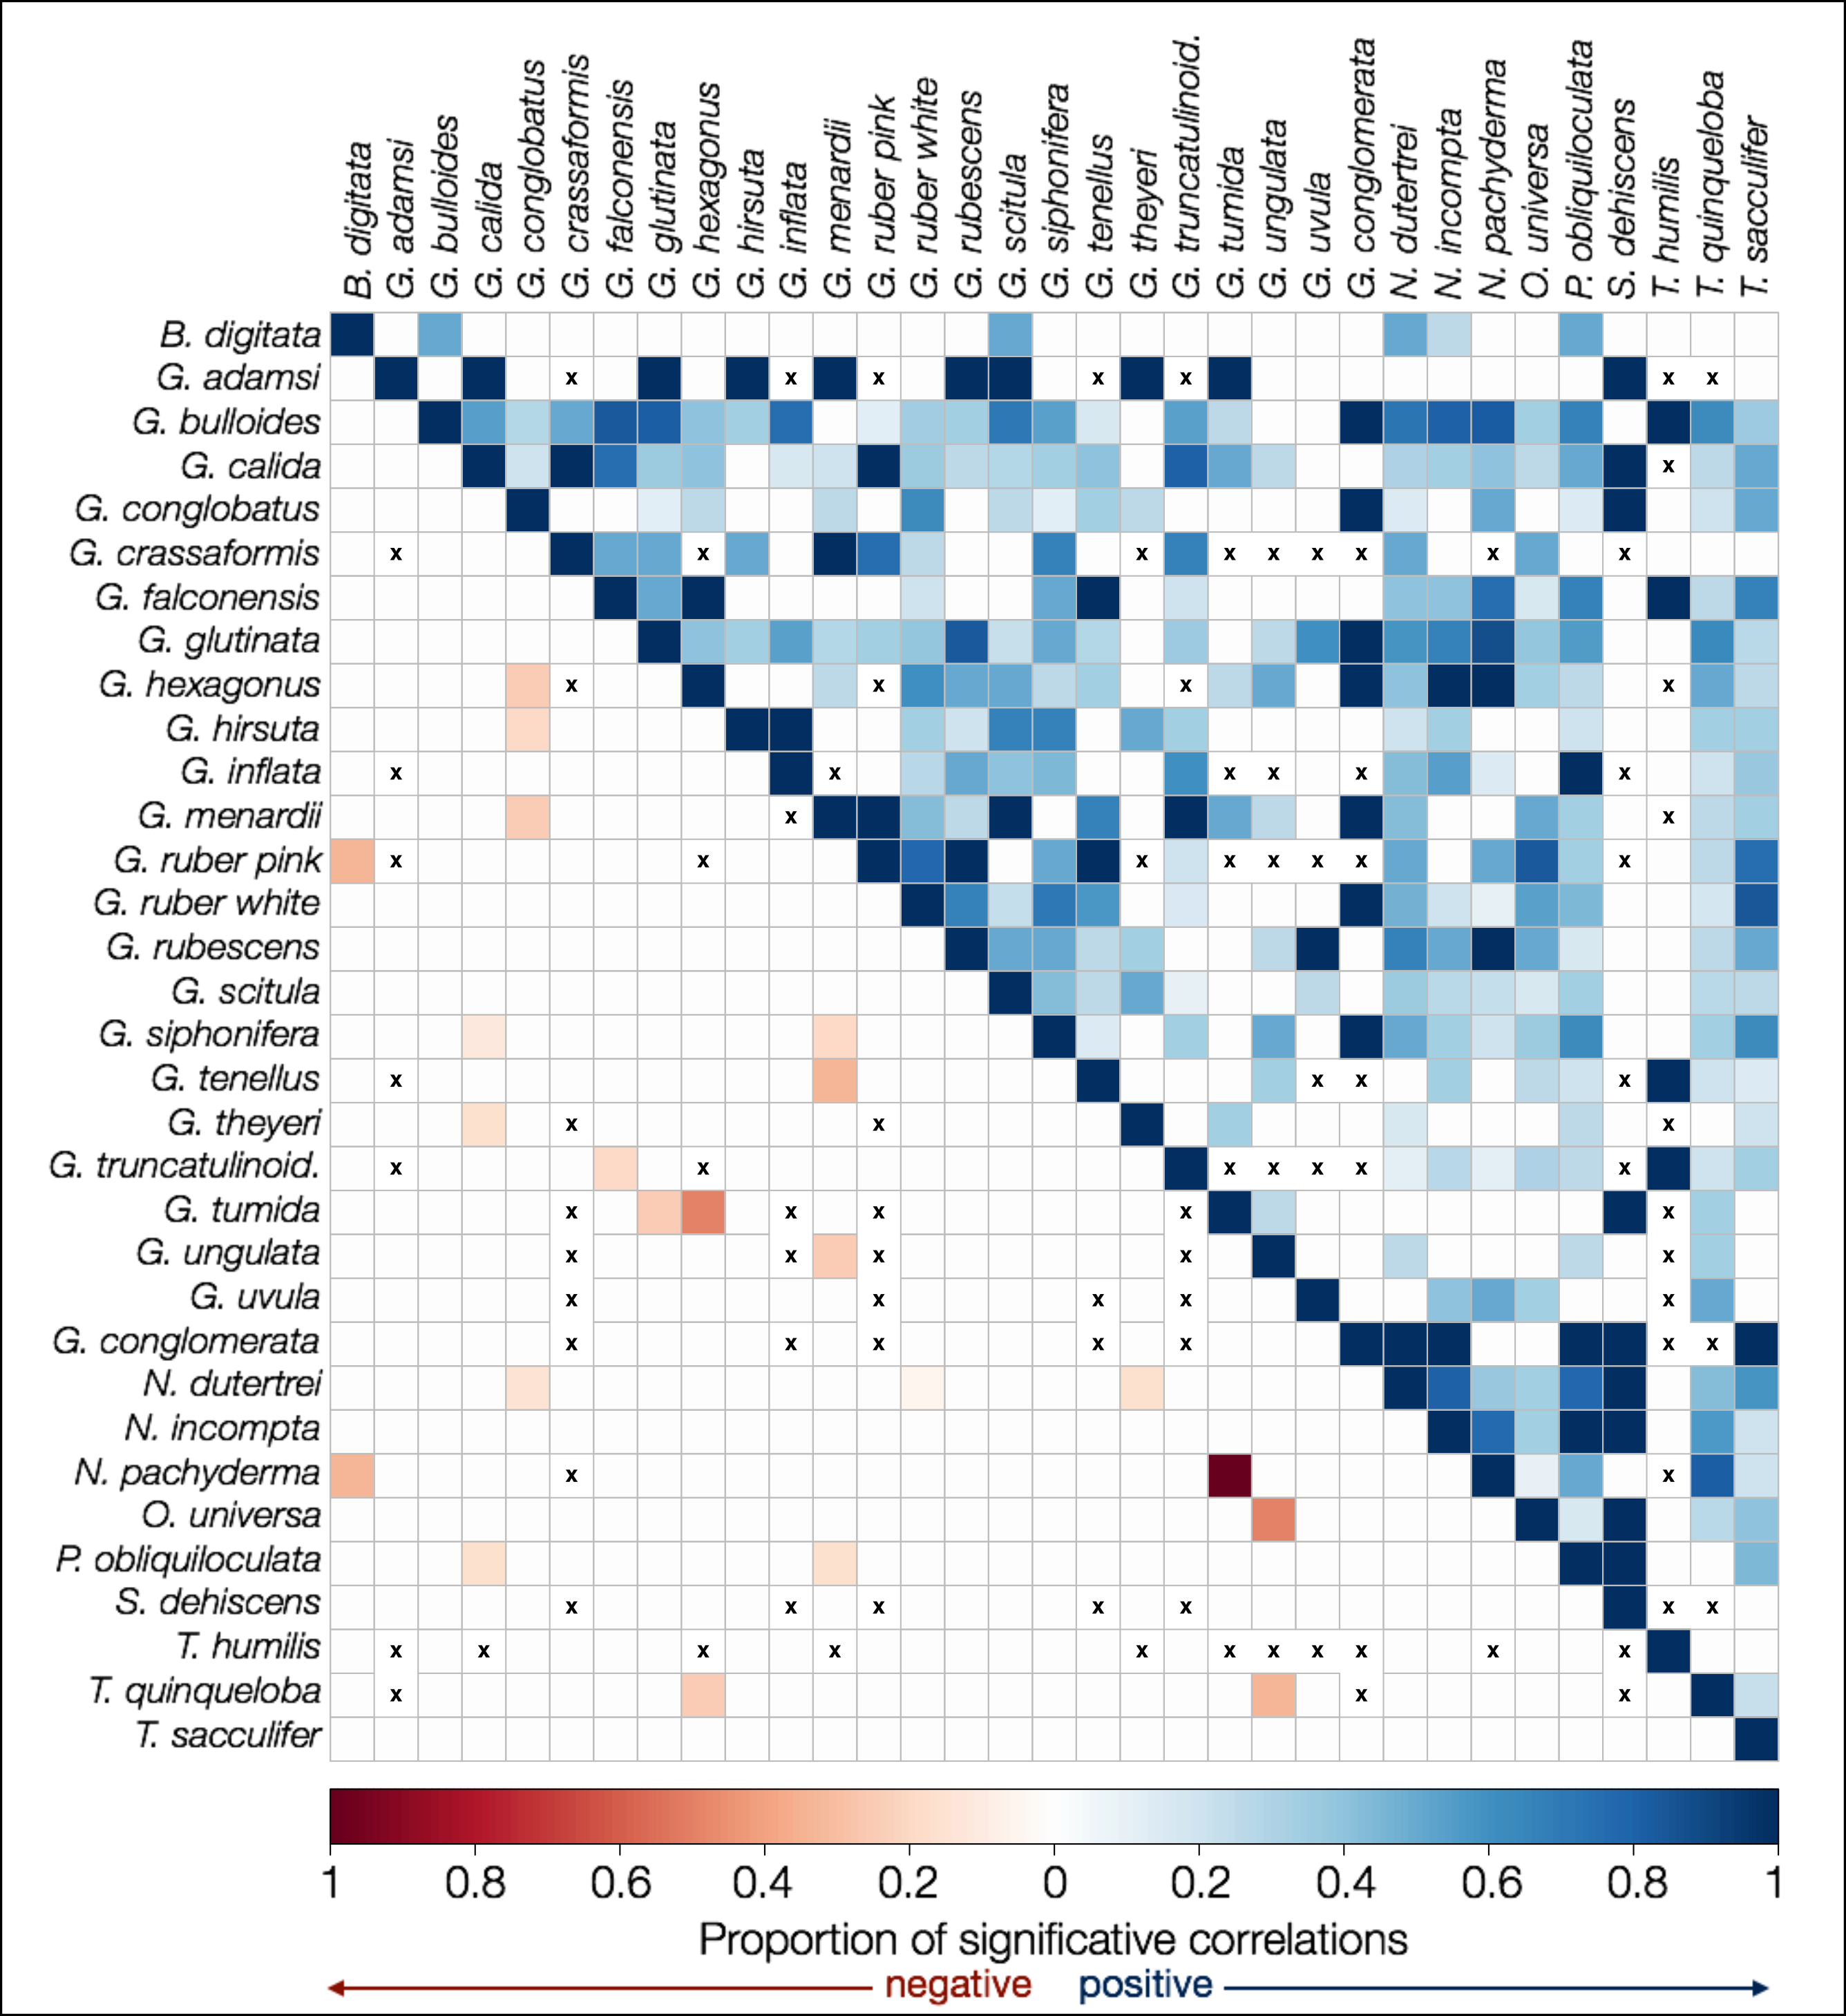
\includegraphics[width=0.8\textwidth]{traps_correlation_low.png}
\caption{\label{fig:corr_prop} Proportion of significant positive (upper triangle, blue) and negative (lower triangle, red) correlations between first differences of time-series in which both species occur. White squares represent species pairs that co-occur but showed no significant positive and/or negative correlation. The black crosses indicate species pairs that did not co-occur.}
\end{figure}
